%! Author = Mina Zarifi
%! Date = 10/13/2020

%!TEX TS-program = xelatex
\documentclass[10pt,A4]{article}

\usepackage[utf8]{inputenc}
\usepackage{xstring,xifthen}
\usepackage{tikz}
\usepackage{lipsum}
\usepackage{graphicx}
\usepackage{array}
\usepackage{tabularx}
\usepackage{moresize}
\usepackage{fancyhdr}
\usepackage{paracol}
\usepackage{transparent}
\usepackage{xcolor}
\usepackage[hidelinks]{hyperref}

\usepackage[a4paper]{geometry}
\geometry{top=1cm, bottom=2cm, left=0.3cm , right=0.3cm}
\pagestyle{empty}
\setlength{\parindent}{0mm}

\newcolumntype{x}[1]{%
>{\raggedleft\hspace{0pt}}p{#1}}%


%-----------------------------fonts-------------------------
%\ProvidesPackage{winfonts}
%\renewcommand{\encodingdefault}{T1}
\RequirePackage{textcomp}
\usepackage{fontspec}
\setmainfont{Times}
\setsansfont{Tahoma}

\definecolor{darkcol}{RGB}{ 70, 70, 70 }
\definecolor{lightcol}{RGB}{245,245,245}
\definecolor{progressclr}{RGB}{129,95,49}
\definecolor{titleNclr}{RGB}{181,129,79}
\definecolor{rulerclr}{RGB}{204,183,171}
\definecolor{linkclr}{RGB}{98,98,98}

\newcommand{\mpwidth}{\linewidth-\fboxsep-\fboxsep}

%----------CV Skills-----------------

\newcommand{\cvskill}[2] {
\begin{tabular*}{1\mpwidth}{p{0.70\mpwidth}  r}
    \textcolor{black}{\textbf{#1}} \\
\end{tabular*}%

\hspace{4pt}
\begin{tikzpicture}[scale=1,rounded corners=2pt,very thin]
    \fill [lightcol] (0,0) rectangle (0.70\mpwidth, 0.15);
    \fill [progressclr] (0,0) rectangle (#2\mpwidth, 0.15);
\end{tikzpicture}%
}
%---CV LIST--------------


\newcommand{\cvlist}[1] {
\begin{itemize}{#1}\end{itemize}
}


%----------------CV TEXT---------------------

\newcommand{\cvtext}[1] {
\begin{tabular*}{1\mpwidth}{p{0.98\mpwidth}}
    \parbox{1\mpwidth}{#1}
\end{tabular*}
}


%------------------CV SECTION----line title bellow--------------------

\newcommand{\cvsection}[1] {
\vspace{14pt}
\cvtext{
\textbf{\LARGE{\textcolor{titleNclr}{\uppercase{#1}}}}\\[-3pt]
\textcolor{rulerclr}{ \rule{0.25\textwidth}{2pt} } \\
}
}

%--------------Language-------------------------

\newcommand{\Language}[2] {
\begin{tabular*}{1\mpwidth}{p{0.72\mpwidth}  r}
    \textcolor{black}{\textbf{#1}} \\
\end{tabular*}%

\hspace{4pt}
\begin{tikzpicture}[scale=1,rounded corners=2pt,very thin]
    \fill [lightcol] (0,0) rectangle (1\mpwidth, 0.15);
    \fill [progressclr] (0,0) rectangle (#2\mpwidth, 0.15);
\end{tikzpicture}%
}

%-------------------work experience------------------------------

\newcommand{\cvevent}[5] {


\parbox{\mpwidth}{
\begin{tabular*}{1\mpwidth}{p{0.72\mpwidth}  r}
    \textcolor{black}{\large{#2}} & \colorbox{white}{\makebox[0.25\mpwidth]{\textcolor{black}{\textbf{#1}}}} \\
    \textcolor{black}{\textbf{#3}} & \\
\end{tabular*}\\[8pt]

\ifthenelse{\isempty{#4}}{}{
\cvtext{#4}\\
}
}

\ifthenelse{\isempty{#5}}{}{
\vspace{9pt}
{#5}
}

}
\vspace{14pt}

%-------------------- CV META EVENT--------------------------
\newcommand{\cvmetaevent}[3] {

\ifthenelse{\isempty{#1}}{}{
\textcolor{darkcol} {\cvtext{\textbf{#1}} \vspace{12pt} }

}

\ifthenelse{\isempty{#2}}{}{
\cvtext{{ \textcolor{darkcol} {#2} }}\\
}

\cvtext{#3}\\[12pt]
}

%-----------------DOCUMENT CONTENT-----------------------------------------
\begin{document}
    \columnratio{0.31}
    \setlength{\columnsep}{2.3em}
    \setlength{\columnseprule}{2pt}
    \colseprulecolor{rulerclr}
    \begin{paracol}{2}
        \begin{leftcolumn}

%-----------------------META IMAGE-----------------------------------

            \begin{tikzpicture}
                \node[circle ,draw=rulerclr,thin]{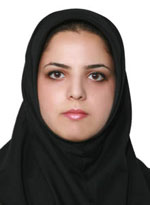
\includegraphics[width=0.58\columnwidth]{zarifi.jpg}};
                \vspace{-9cm}
            \end{tikzpicture}

%--------------profile------------------------------
            \cvsection{PROFILE}
            \cvmetaevent
            {Gender: Female \\
            Nationality: IRANIAN \\
            Birth Date: 1/6/1986}
            {Software engineer with a strong background
            in design and development on
            .NET platform for more than 8 years.
            }
%--------EDUCATION------------------------------------
            \cvsection{EDUCATION}
            \cvmetaevent
            {Bachelor of Science :}
            {from Qazvin Azad University in\\[2pt] Software Engineering from\\[2pt]
            September 2006 to September 2010.}
            %-------------------------META SKILLS----------------------------

            \cvsection{Languages}

            \Language{English} {0.65} \\[-2pt]

            \Language{Persian}  {1} \\[-2pt]


            \null\null

%----------------------Contact------------------------------------
            \cvsection{CONTACT}

            \cvtext{

            \textbf{\textcolor{black} {Email}}: \href{mailto:m101.zarifi@gmail.com}{\color{linkclr}{m101.zarifi@gmail.com}}\\[3pt]
            \textbf{\textcolor{black} {Mobile} }: +98912 666 22 62\\[3pt]
            \textbf{\textcolor{black} {LinkedIn}}: \href{linkedin.com/in/mina-zarifi-7b6a701b5}{\color{linkclr}{linkedin.com/in/mina-zarifi-7b6a701b5}}  \\[3pt]
            \textbf{\textcolor{black} {Address}}: Number 36-Sabooniha \\
            STREET-SHAHR RAY-Tehran-IRAN
            }

            \vfill


        \end{leftcolumn}
        \begin{rightcolumn}

%--------------TITLE  HEADER----------------------------

            \fcolorbox{white}{darkcol}{\begin{minipage}[c][4.3cm][c]{1\mpwidth}
                                           \begin {center}
                                               \HUGE{ \textbf{ \textcolor{white}{ \uppercase{ MINA ZARIFI } } } } \\[-24pt]
                                               \textcolor{white}{ \rule{0.30\textwidth}{1.20pt} } \\[4pt]
                                               \large{ \textcolor{white} {SOFTWARE ENGINEER} }
                                           \end {center}
            \end{minipage}} \\[14pt]

%-------------------WORK EXPERIENCE-----------------------

            \vfill
            \cvsection{WORK EXPERIENCE}
            \cvevent
            {Dec 2010 - Apr 2017}
            {TEHRAN MUNICIPALITY ICT CENTER}
            {Developer and Designer}
            {Model Components and Modules of Data Center and Edit them for Example Line, Rack, Server ,Hardware ,DB and Applications Create Report to Users with Crystal Report , design DB with oracle .}
            {}

            \vspace{0.55in}


            \cvevent
            {Apr 2017 - Present}
            {TEHRAN MUNICIPALITY ICT CENTER}
            {Administrator}
            {Backup DB of Tehran municipality ICT Center and keep them up in Home Office and Studying new technologies.}
            {}
            \vspace{0.58in}
\null
%---------------------certification-------------------------------
            \cvsection{CERTIFICATIONS}

            \cvevent
            {Feb 2014}
            {VANDA RAAD SAMANEH -TEHRAN -IRAN}
            {ORACLE Data Guard}
            {}
            {}
            \vspace{0.25in}
            \cvevent
            {Feb 2014 -Mar 2014}
            {TEHRAN Municipality ICT Center}
            {ITIL Course}
            {}
            {}
            \vspace{0.25in}
            \cvevent
            {Jun 2015}
            {ABSHAR DATA PROCESSING, TEHRAN, IRAN}
            {Information Security Management System (ISMS) Fundamentals }
            {}
            {}
            \vspace{0.25in}
            \cvevent
            {Aug 2015}
            {CANDO Company, TEHRAN, IRAN}
            {Implementing a Data Warehouse with Microsoft SQL Server 2012}
            {}
            {}
            \vfill\null\null

            \newpage
        \end{rightcolumn}
    \end{paracol}

    \newpage


    \newcolumntype{C}{>{\centering\arraybackslash}b{0.65\paperwidth}}
    \newcolumntype{L}{>{\centering\arraybackslash} m{0.29\paperwidth}}

    \begin{table}
        \centering
        \begin{tabular}{ L C }
            \centering
            \begin{tikzpicture}
                \node[circle ,draw=rulerclr,thin]{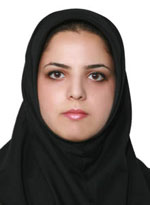
\includegraphics[width=0.17\columnwidth]{zarifi.jpg}};

            \end{tikzpicture} &

            \fcolorbox{white}{darkcol}{\begin{minipage}[c][4.8cm][c]{1\mpwidth}
                                           \begin {center}
                                               \HUGE{ \textbf{ \textcolor{white}{ \uppercase{ MINA ZARIFI } } } } \\[-24pt]
                                               \textcolor{white}{ \rule{0.30\textwidth}{1.20pt} } \\[4pt]
                                               \large{ \textcolor{white} {SOFTWARE ENGINEER} }
                                           \end {center}
            \end{minipage}} \\

        \end{tabular}
        \newline
        \newline

    \end{table}

    \cvsection{PROGRAMMING SKILLS}

    \cvskill{C\#}  {0.64} \\[6pt]
    \cvskill{Asp.NET}  {0.64} \\[6pt]
    \cvskill{HTML5}  {0.63} \\[6pt]
    \cvskill{CSS3}  {0.63} \\[6pt]
    \cvskill{JavaScript}  {0.60} \\[6pt]
    \cvskill{BootStrap4}  {0.50} \\[6pt]
    \cvskill{JQuary}  {0.54} \\[6pt]
    \cvskill{Nhibernate}  {0.57} \\[6pt]
    \cvskill{Python}  {0.51} \\[6pt]
    \cvskill{Angular}  {0.52} \\[6pt]
    \cvskill{Node.js}  {0.51} \\[6pt]
    \cvskill{Oracle PL/SDQL Development}  {0.57} \\[6pt]
    \cvskill{SQLSERVER}  {0.62} \\[6pt]
    \cvskill{CrystalReport}  {0.65} \\[6pt]
    \cvskill{\LaTeX}  {0.60} \\[6pt]


\end{document}


